\documentclass{article}

% Use the [final] option for camera-ready version as per template comments
% If submitting a preprint to arXiv, change 'final' to 'preprint'
\usepackage[final]{neurips_2024}

% to avoid loading the natbib package, add option nonatbib:
% usepackage[nonatbib]{neurips_2024} % Commented out as citations are desired

\usepackage[utf8]{inputenc} % allow utf-8 input - Handled natively by XeTeX/LuaTeX, but kept for compatibility
\usepackage[T1]{fontenc}    % use 8-bit T1 fonts
\usepackage{hyperref}       % hyperlinks
\usepackage{url}            % simple URL typesetting
\usepackage{booktabs}       % professional-quality tables
\usepackage{amsfonts}       % blackboard math symbols
\usepackage{nicefrac}       % compact symbols for 1/2, etc.
\usepackage{microtype}      % microtypography
\usepackage{xcolor}         % colors
\usepackage{amsmath}        % Math environments and commands
\usepackage{algorithm}      % Algorithm float environment
\usepackage{algpseudocode}  % Pseudocode environment
\usepackage{enumitem}       % For customizing lists like enumerate - Use \begin{itemize}[leftmargin=*, noitemsep, topsep=0pt] for tighter lists
\usepackage{graphicx}       % For including images
\usepackage{caption}        % For customizing captions
\usepackage{subcaption}     % For subfigures
\usepackage{makecell}       % For multi-line table cells

% NOTE: The neurips_2024.sty file already loads 'natbib'.
% Explicitly loading it again can cause conflicts or redundancy.
% Removed: \usepackage{natbib} % This was already commented out, confirming the original code is correct here.

% The neurips_2024 style typically defaults to author-year or a specific numeric style.
% You might need to check the .sty file or its documentation for citation style options.
\bibliographystyle{abbrvnat}

% Update Title and Author information
\title{Beyond Sentiment: Classifying Evaluative vs. Non-evaluative Text using LLM-Labeled Data and Adapter Fine-tuning}

% The \author macro works with any number of authors. There are two commands
% used to separate the names and addresses of multiple authors: \And and \AND.
%
% Using \And between authors leaves it to LaTeX to determine where to break the
% lines. Using \AND forces a line break at that point. So, if LaTeX puts 3 of 4
% authors names on the first line, and the last on the second line, try using
% \AND instead of \And before the third author name.

\author{%
Bomin Zhang\\
University of Maryland \\ % Corrected University spelling
College Park, MD 20742 \\
\texttt{bominz2@umd.edu} \\
% Add course and date here if needed, maybe as a footnote to the title or after the abstract.
% For example:
% \thanks{Course: Big Data Analytics - Final Project. Date: May 8, 2025}
}

\begin{document}

\maketitle

\begin{abstract}
This paper addresses the task of classifying text based on a nuanced definition: distinguishing evaluative judgments (evaluative) from non-evaluative statements and descriptions of direct experience (non-evaluative). This challenge stems from the lack of large-scale labeled datasets aligned with this specific distinction, which goes beyond traditional sentiment analysis and broad subjectivity detection. We leverage Large Language Models (LLMs) to generate synthetic training data. Parameter-efficient fine-tuning (PEFT), specifically LoRA, is employed on a pre-trained language model (DistilRoBERTa-base) for the classification task. LoRA fine-tuning performance is compared against standard direct fine-tuning on the 20 Newsgroups dataset, using a partially human-reviewed test set for robust evaluation. Findings indicate some success and suggest avenues for further research on this novel semantic analysis feature.
\end{abstract}


\section{Introduction}
\label{sec:introduction}

\textbf{Hume's guillotine}, or the \textbf{Is-Ought Problem}, highlights a philosophical distinction where evaluative conclusions cannot strictly be inferred from purely factual statements. Extending this, \textbf{evaluation} and \textbf{description} can be seen as operating on parallel systems in formal reasoning. Evaluation doesn't alter the physical world, while physical conditions inform, but don't modify, the evaluative system itself. This philosophical divide underscores a need in NLP to differentiate text making judgments from text describing facts or experiences. Traditional sentiment analysis focuses on polarity, and broad subjectivity detection includes feelings and experiences alongside judgments, leaving the specific distinction between evaluative judgments and non-evaluative text less explored. We clarify these distinctions next.

\section{Definitions and Comparison of Classification Axes}
\label{sec:definitions_comparison}

We define and compare three key axes for text classification relevant to this work:

\subsection{Objective vs. Subjective (Broad)}
\textbf{Objective:} Verifiable facts, external reality, independent of personal feelings.
\textbf{Subjective (Broad):} Internal states, personal feelings, experiences, beliefs, opinions, judgments. Includes anything not purely objective.

\subsection{Sentiment (Positive/Negative/Neutral)}
\textbf{Sentiment:} Emotional tone or polarity (Positive, Negative, Neutral) towards a subject.

\subsection{Evaluative vs. Non-evaluative (This Work)}
\textbf{Evaluative:} Text expressing an \textit{evaluative judgment, stance, argument, or assessment} about a subject. Considered a \textit{subset} of broad subjective text in this context.
\textbf{Non-evaluative:} Text that is either a verifiable \textit{objective fact/report} OR a \textit{subjective report of personal experience, feeling, or non-evaluative description} without a generalized evaluative judgment.

\subsection{Comparison of Axes}
\label{sec:comparison}

These axes capture distinct aspects. Table \ref{tab:evaluative_comparison} briefly illustrates the difference between the Evaluative/Non-evaluative axis and the other two.

\begin{table}[htbp]
\centering
\caption{Comparison of Evaluative/Non-evaluative with Sentiment and Objective/Subjective}
\label{tab:evaluative_comparison}
\begin{tabular}{p{3cm} | p{5.5cm} | p{5.5cm}}
\toprule
Axis / Class & \textbf{Evaluative} & \textbf{Non-evaluative} \\
\midrule
\textbf{Sentiment (Pos/Neg)} &
\makecell[l]{Ex: "Best pizza in town." (Eval, Pos) \\ Ex: "Service appalling." (Eval, Neg)} &
\makecell[l]{Ex: "Heartbroken by news." (Pure feeling, implies Neg) \\ Ex: "Sales up 30\%." (Objective, implies Pos)} \\
\midrule
\textbf{Sentiment (Neutral)} &
\makecell[l]{Ex: "Comprehensive, dry analysis." (Eval, Mixed/Neutral) \\ Ex: "Necessary step, but fails..." (Eval, Mixed/Neutral)} &
\makecell[l]{Ex: "Sky is blue." (Objective, Neutral) \\ Ex: "Felt sleepy." (Pure experience, Neutral)} \\
\midrule
\textbf{Objective} & \textit{Contradictory.} Evaluative is subjective. & Ex: "Water boils at 100C." (Objective) \\
\midrule
\textbf{Subjective (Broad)} &
\makecell[l]{Ex: "Book incredibly insightful." (Judgment) \\ Ex: "Argument relies on flawed logic." (Evaluative stance)} &
\makecell[l]{Ex: "Feel under weather." (Pure feeling) \\ Ex: "Believe tomorrow sunny." (Belief)} \\
\bottomrule
\end{tabular}
\end{table}

This comparison shows the Evaluative/Non-evaluative axis focuses uniquely on the presence of \textbf{evaluation} or \textbf{judgment}.

\subsection{Importance of the "Evaluativeness" Axis}
\label{sec:why_evaluativeness}
Separating evaluative from descriptive/factual content aids NLP applications by enhancing interpretability, filtering bias in information retrieval, and improving automated reasoning.

\subsection{Research Challenge}
A key challenge is the lack of large datasets explicitly labeled per this nuanced definition, unlike sentiment or broad subjectivity data.

\subsection{Adopted Methodology}
\label{sec:methodology_overview}
We address this by leveraging LLMs (GPT-4.1 mini) for synthetic training data generation via careful prompt engineering \citep{tan2024largelanguagemodelsdata}. We apply parameter-efficient fine-tuning (PEFT), specifically LoRA \citep{hu2021LoRAlowrankadaptationlarge}, on DistilRoBERTa-base \citep{sanh2020distilbertdistilledversionbert}. This is compared against standard direct fine-tuning. Training and evaluation use data from the 20 Newsgroups dataset \citep{twenty_newsgroups_113} with a partially human-reviewed test set.

Contributions:
\begin{enumerate}[label=\arabic*., leftmargin=*, noitemsep, topsep=0pt]
\item Defining and tackling the evaluative vs. non-evaluative classification based on a novel nuance.
\item Demonstrating LLM-assisted labeling effectiveness via prompt engineering for synthetic data.
\item Evaluating LoRA vs. direct fine-tuning of DistilRoBERTa-base on LLM-labeled data.
\item Analyzing model performance across dataset topics.
\end{enumerate}

\section{Related Work}
\label{sec:related_work}
Relevant areas include:
\subsection{Sentiment Analysis}
\label{sec:related_work:sentiment}
Focuses on polarity and broad subjectivity \citep{liu2012sentiment}.

\subsection{Subjectivity Detection}
\label{sec:related_work:subjectivity}
Distinguishes subjective from objective \citep{liu2012sentiment}, using corpora like MPQA \citep{wiebe2005annotating}. However, its "subjective" is broader, including experiences/beliefs without explicit judgment, differing from this work's 'evaluative'.

\subsection{LLMs for Data Annotation}
\label{sec:related_work:llm_annotation}
LLMs aid annotation for tasks lacking data \citep{tan2024largelanguagemodelsdata}. Prompt engineering is crucial \citep{brown2020language}. LLM bias/noise must be considered.

\subsection{Parameter-Efficient Fine-Tuning (PEFT)}
\label{sec:related_work:peft}
Trains a small fraction of parameters to adapt large models efficiently \citep{han2024parameterefficientfinetuninglargemodels}. LoRA \citep{hu2021LoRAlowrankadaptationlarge} injects low-rank matrices. PEFT saves time, memory, and storage \citep{pfeiffer2020AdapterHub, peft}.

\section{Methodology}
\label{sec:methodology}
\subsection{Data Source and Preparation}
\label{sec:methodology:datasource}
Using the 20 Newsgroups dataset \citep{twenty_newsgroups_113} due to its diverse topics (Figure \ref{fig:20ng_topics}). Preprocessing included removing headers, footers, and segmenting text.

\begin{figure}[h!]
\centering
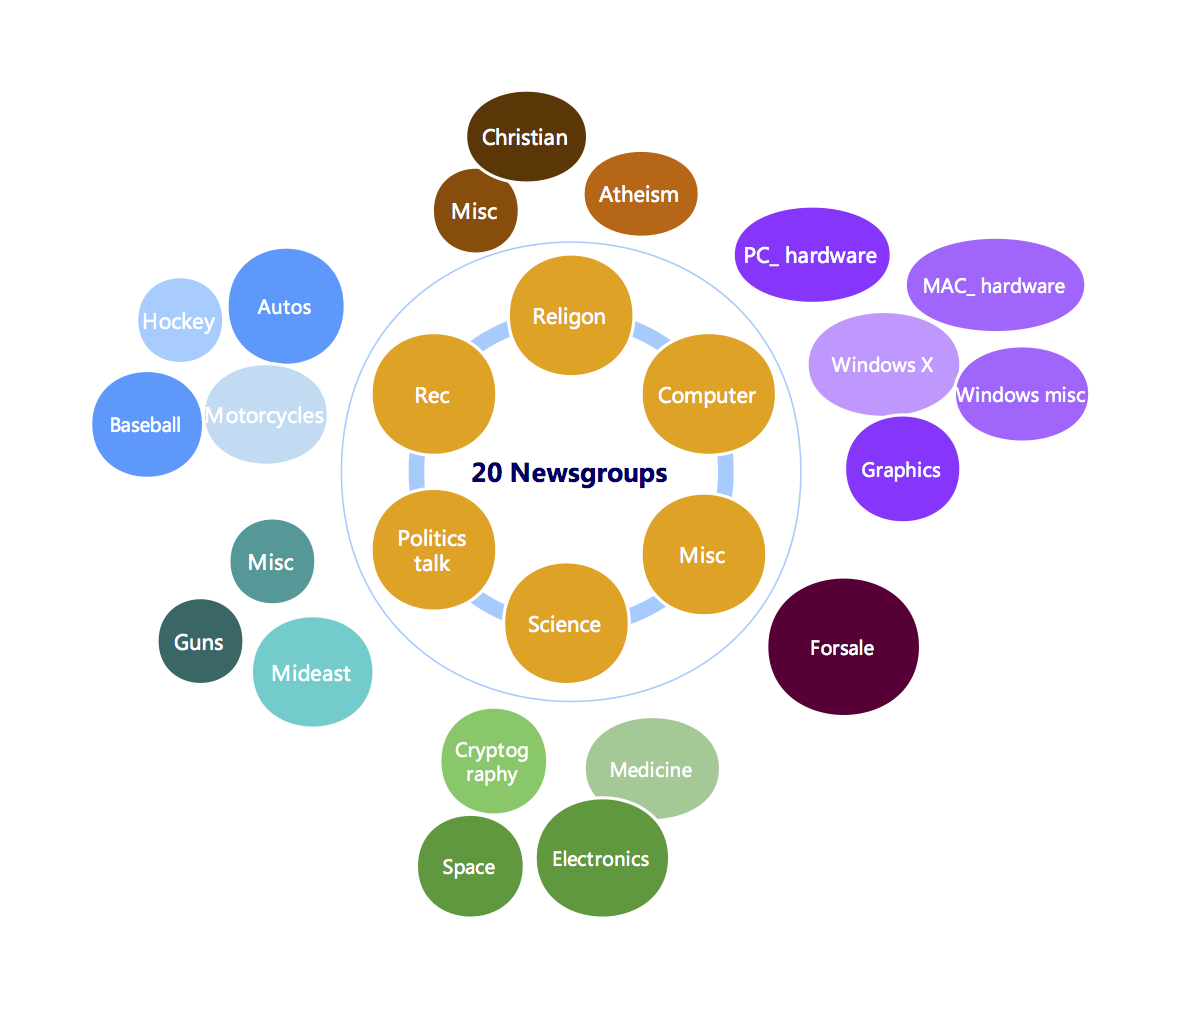
\includegraphics[width=0.6\linewidth]{attachments/20_news.png} % Reduced width slightly
\caption{Distribution of documents across the 20 newsgroup topics.}
\label{fig:20ng_topics}
\end{figure}

\subsection{Data Labeling Strategy (LLM-Assisted)}
\label{sec:methodology:llm_labeling}
GPT-4.1 mini generated labels for 10,000 sampled snippets. Prompts included precise definitions and examples. LLM noise exists; manual review of 500 samples found ~9 incorrect labels and ~9 correct labels with incorrect reasoning. More details in Appendix \ref{sec:appendix}.

\subsection{Model Architecture}
\label{sec:methodology:architecture}
`DistilRoBERTa-base` \citep{sanh2020distilbertdistilledversionbert}, a distilled RoBERTa model, was used with a linear classification head.

\subsection{Fine-tuning Strategies}
\label{sec:methodology:finetuning}
\begin{itemize}[leftmargin=*, noitemsep, topsep=0pt]
\item \textbf{Direct Fine-tuning:} Standard approach, trains substantial model parameters.
\item \textbf{LoRA Fine-tuning:} PEFT method, freezes base model and trains low-rank matrices injected into transformer layers.
\end{itemize}

\section{Experimental Setup}
\label{sec:experimental_setup}
From ~50,000 pruned texts, 10,000 were sampled preserving topic distribution. This split into 80\% (8,000) training and 20\% (2,000) test sets, LLM-labeled. Labels encoded: "evaluative", "non-evaluative".

Models fine-tuned on `DistilRoBERTa-base` using Hugging Face Transformers/PyTorch and `peft`.
Hyperparameters: lr = $2 \times 10^{-5}$, Batch size = 200, Epochs = 10.
LoRA parameters: rank $r = 16$, scaling $\alpha = 64$, dropout $d = 0.05$. Trains 1,034,498 parameters (1.24\% of base model).
Hardware: Single RTX2080Ti (11GB).
Evaluation metrics: F1 Score (primary), Accuracy, Precision, Recall. Also F1 per topic.

\section{Results}
\label{sec:results}
Evaluated on 2000-sample test set.

\subsection{Overall Performance}
\label{sec:results:overall}
Table \ref{tab:overall_metrics} shows performance for the 'evaluative' class.

\begin{table}[htbp]
    \centering
    \caption{Overall Performance ('Evaluative' Class)}
    \label{tab:overall_metrics}
    \small % Reduced font size for table
    \begin{tabular}{l c c c c}
        \toprule
        Model & Acc. & 'Eval' P & 'Eval' R & 'Eval' F1 \\
        \midrule
        Direct FT & 0.8755 & 0.7845 & 0.7858 & 0.7852 \\
        LoRA FT   & 0.8525 & 0.7536 & 0.7288 & 0.7410 \\
        \bottomrule
    \end{tabular}
\end{table}
Direct fine-tuning outperformed LoRA (0.7852 vs 0.7410 'evaluative' F1), suggesting fuller model adaptation was more effective.

\subsection{Confusion Matrix}
\label{sec:results:confusion_matrix}
Test set has 579 evaluative, 1421 non-evaluative samples.

\begin{figure}[h!]
    \centering
    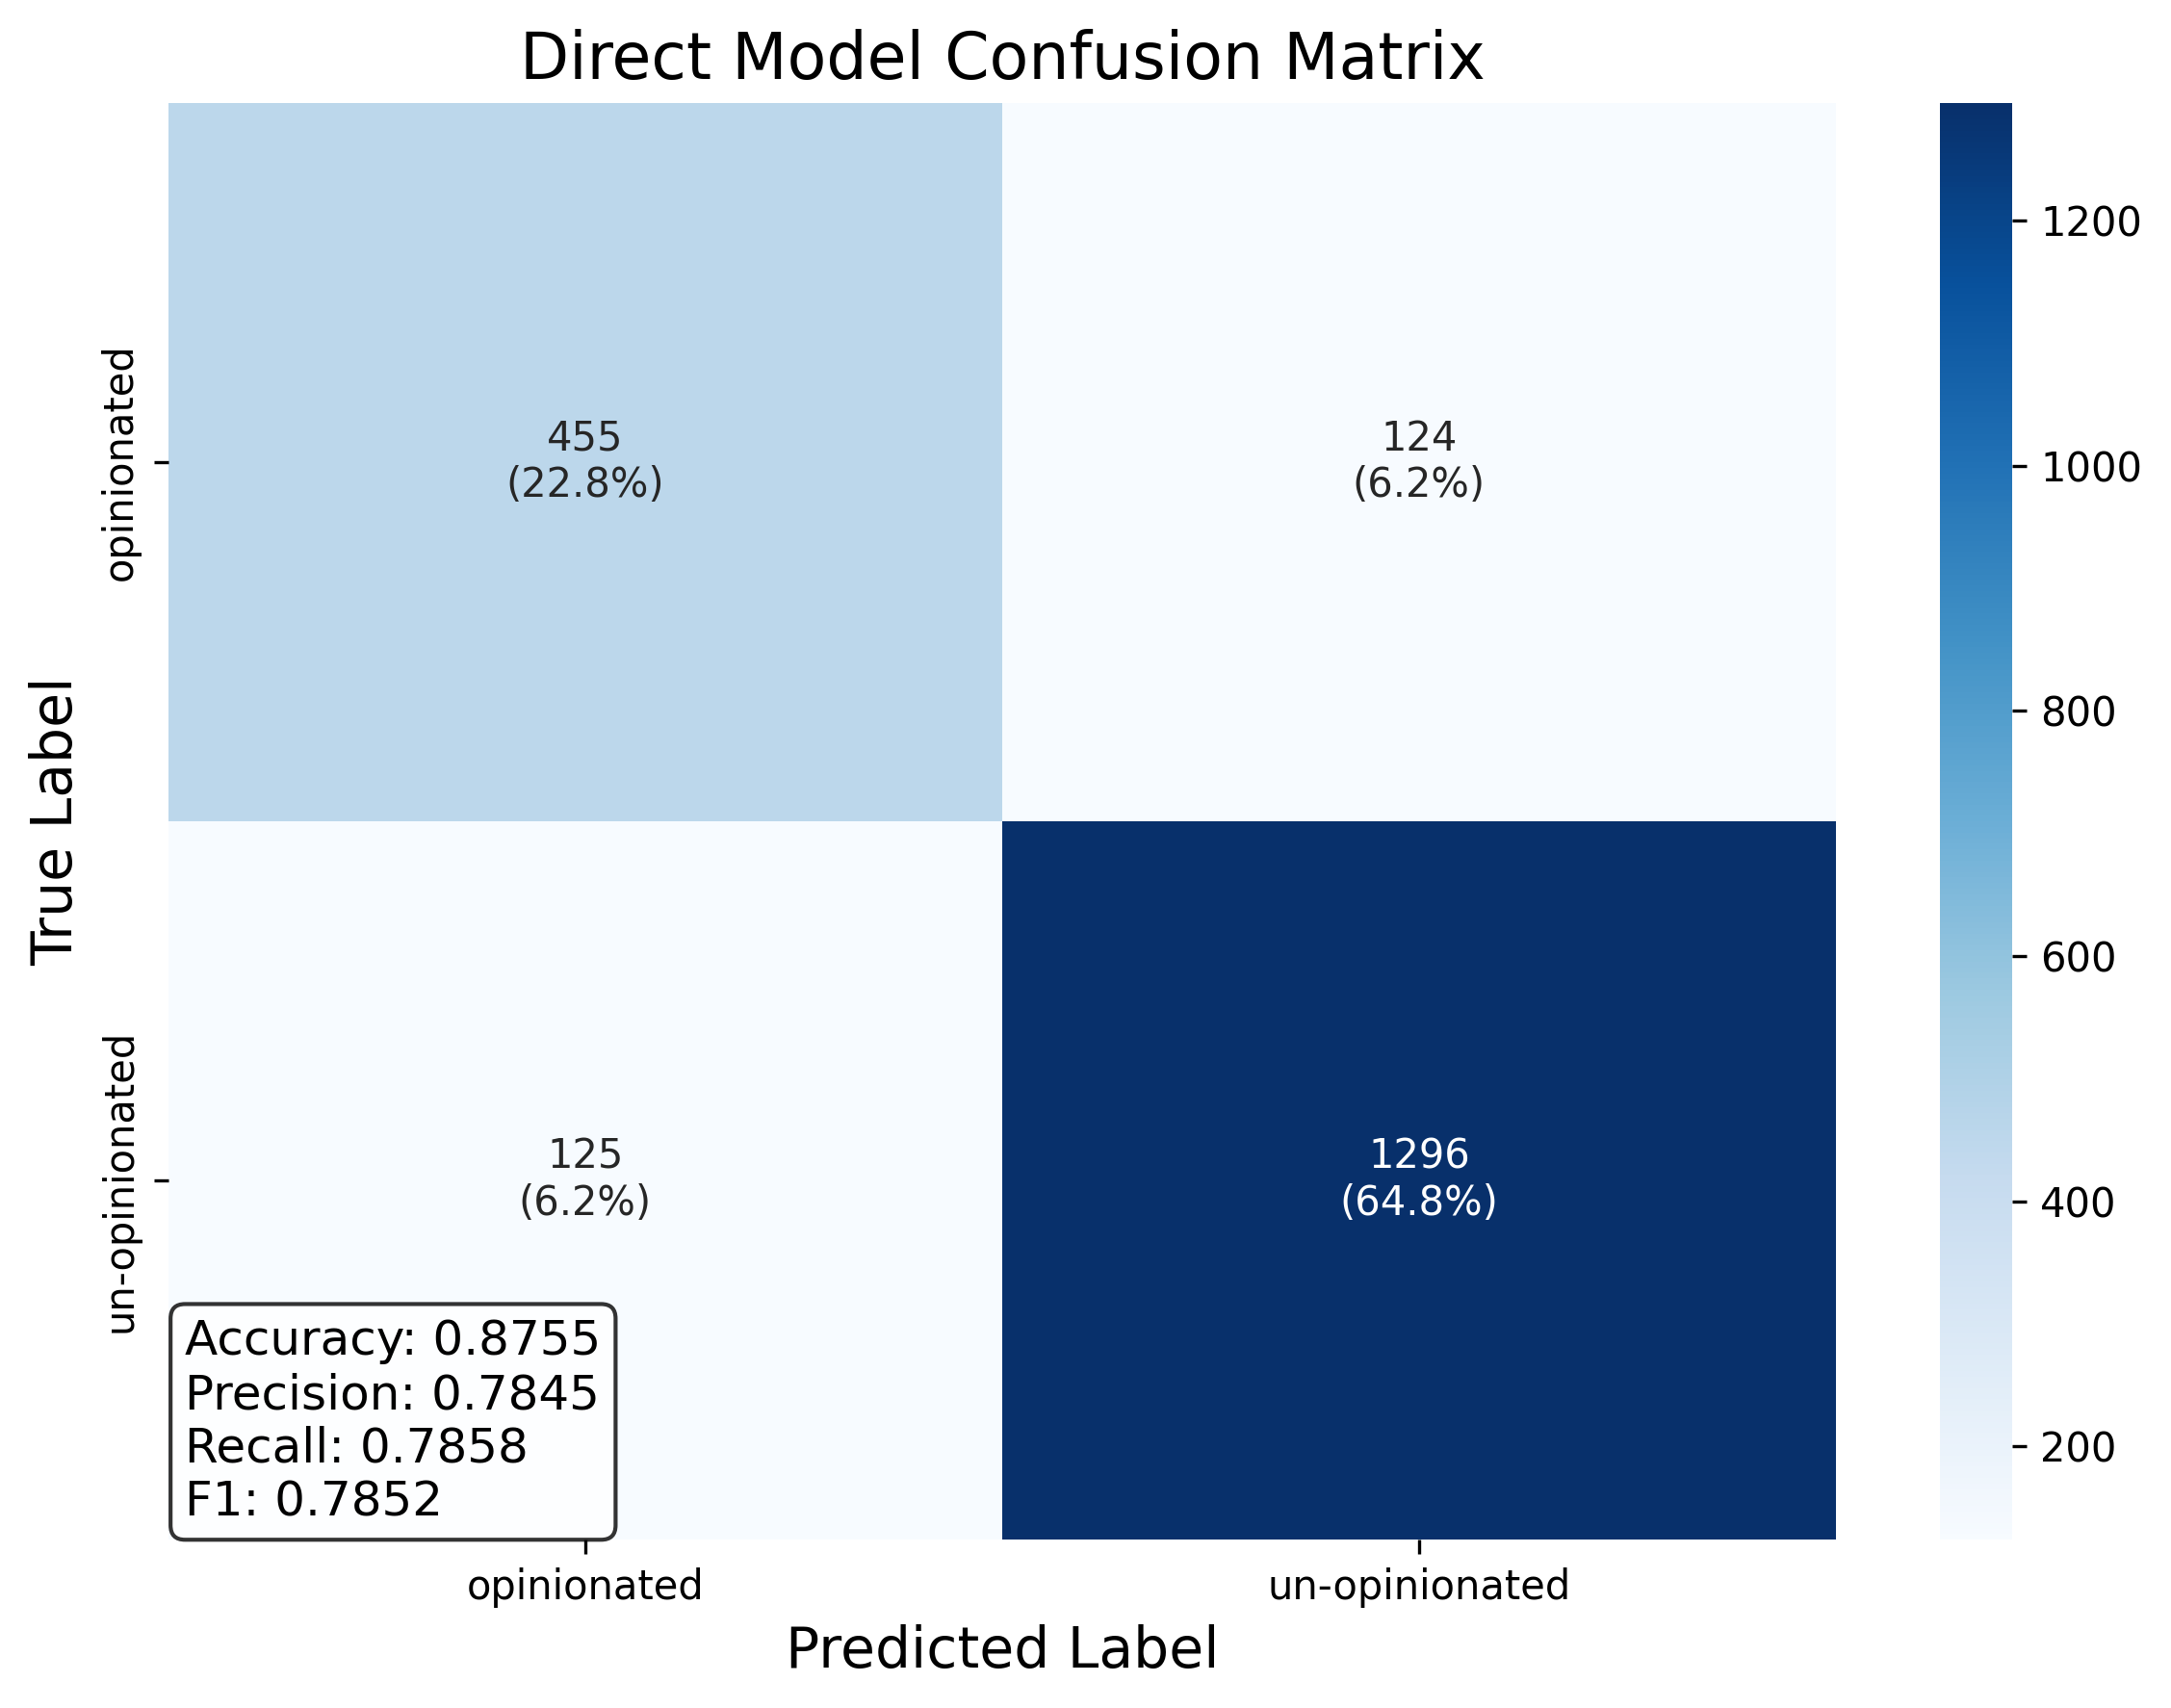
\includegraphics[width=0.45\linewidth]{attachments/confusion_matrix_direct.png} % Reduced width
    \includegraphics[width=0.45\linewidth]{attachments/confusion_matrix_LoRA.png} % Reduced width
    \caption{Confusion Matrices: Direct Model (Left) and LoRA Model (Right) on Test Set}
    \label{fig:confusion_matrices} % Combined figures, updated label
\end{figure}
Figure \ref{fig:confusion_matrices} shows direct FT had fewer misclassifications (FN: 124 vs 157, FP: 125 vs 138). Both show notable False Negatives.

\subsection{Performance by Topic}
\label{sec:results:topic}
Figures \ref{fig:ranked_f1_direct} and \ref{fig:ranked_f1_LoRA} show F1 scores per topic.

\begin{figure}[h!]
    \centering
    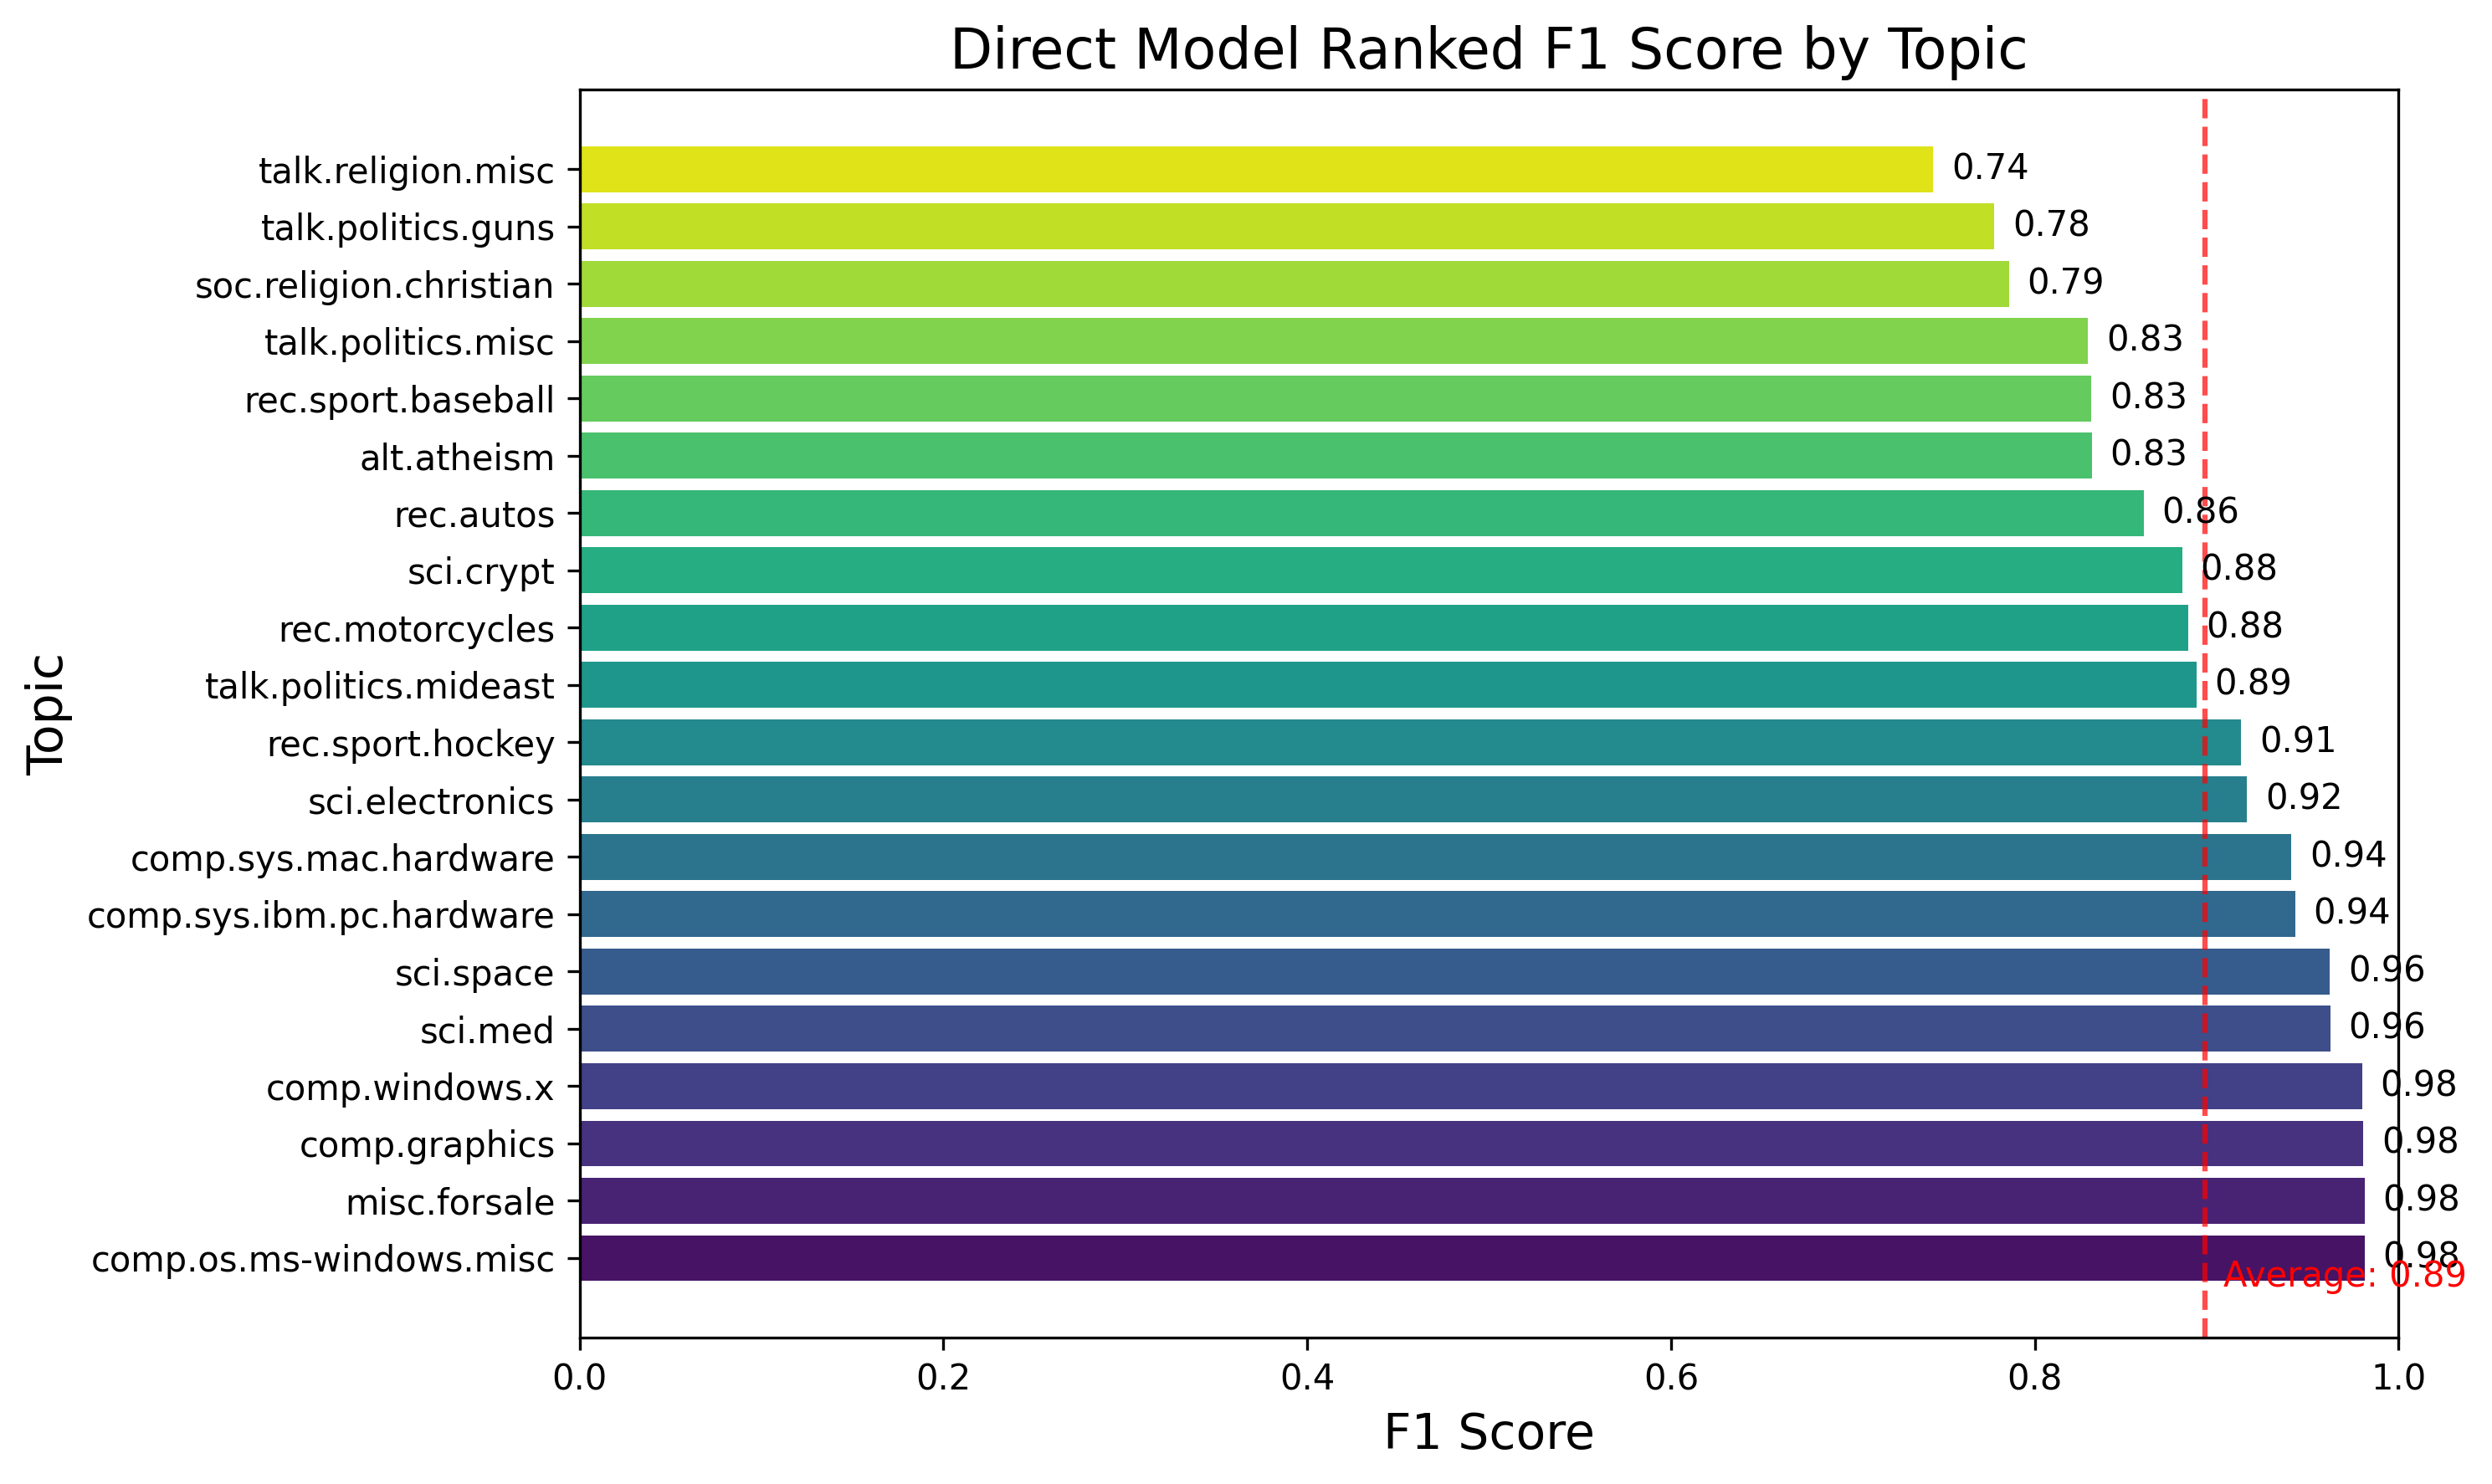
\includegraphics[width=0.9\linewidth]{attachments/ranked_f1_direct.png} % Keep width for readability
    \caption{F1 Scores by Topic for Direct Model}
    \label{fig:ranked_f1_direct}
\end{figure}

\begin{figure}[h!]
    \centering
    \includegraphics[width=0.9\linewidth]{attachments/ranked_f1_LoRA.png} % Keep width for readability
    \caption{F1 Scores by Topic for LoRA Model}
    \label{fig:ranked_f1_LoRA}
\end{figure}
Average F1 is ~0.779 for Direct, ~0.651 for LoRA. LoRA lags more significantly in the lowest-performing topics (`comp.sys.ibm.pc.hardware`, `comp.sys.mac.hardware`, `comp.windows.x`, `talk.religion.misc`), often related to politics/religion which were challenging domains. Topics like `sci.space` and `rec.sport.hockey` had higher scores.

\section{Analysis}
\label{sec:analysis}
Manual analysis confirmed LLM's ability to apply the definition, though errors occurred (~9/500 incorrect labels). Evaluation showed direct FT superior to LoRA, with an 'evaluative' F1 of 0.7852 vs 0.7410. LoRA's parameter efficiency came at a performance cost. Performance varied by topic, highlighting domain dependence; political/religious domains were harder. Close topics showed relatively close results, aligning with previous findings using similar models\footnote{Note: This observation is specific to this experiment and model choice.}.

\section{Limitations and Future Work}
\label{sec:limitations_future_work}
\subsection{Limitations}
\label{sec:limitations}
\begin{itemize}[leftmargin=*, noitemsep, topsep=0pt]
\item LLM training data noise/bias.
\item Definition specificity; not universally applicable.
\item Performance tied to 20 Newsgroups domain.
\item Resource limits restricted hyperparameter tuning, larger models.
\item Binary classification only.
\item Limited human test set size impacts granular analysis robustness.
\item Masked language model (DistilRoBERTa) might not be optimal vs. autoregressive LLMs for nuances.
\end{itemize}

\subsection{Future Work}
\label{sec:future_work}
\begin{itemize}[leftmargin=*, noitemsep, topsep=0pt]
  \item Improve LLM labeling (larger LLMs, advanced prompting).
  \item Expand human data (larger test set, partial training set).
  \item Cross-domain evaluation and adaptation.
  \item Multi-class modeling (Judgment, Fact, Experience).
  \item Comprehensive PEFT comparison.
  \item Explainability: understand features driving classification.
  \item Integrate classifier into larger NLP pipelines.
  \item Leverage existing subjectivity detectors to refine LLM labels.
\end{itemize}

\section{Conclusion}
\label{sec:conclusion}
This study successfully defined and addressed the task of classifying evaluative vs. non-evaluative text using LLM-assisted labeling on the 20 Newsgroups dataset. We compared standard direct fine-tuning with LoRA on DistilRoBERTa-base. Direct fine-tuning achieved an 'evaluative' F1 of 0.7852, outperforming LoRA (0.7410), demonstrating that full model adaptation was more effective for this task's nuanced distinction, despite LoRA's parameter efficiency. Performance varied across topics, highlighting domain challenges. This work contributes a methodology for tackling tasks lacking large datasets via LLMs and introduces a valuable semantic distinction for NLP applications. Future work should refine data quality, expand evaluation, explore multi-class distinctions, and analyze PEFT trade-offs further.

\section{Appendix}
\label{sec:appendix}

\subsection{Manual Analysis of LLM-Generated Labels}
\label{sec:appendix:manual_analysis}
A manual review of 500 LLM-labeled samples was conducted to assess label quality. The analysis confirmed that GPT-4.1 mini was largely capable of applying the specific definition of 'evaluative' vs. 'non-evaluative' provided through prompt engineering. Out of the 500 reviewed samples, approximately 9 samples were identified as having an incorrect classification label assigned by the LLM. A similar number of samples received the correct label but were accompanied by incorrect or questionable reasoning provided by the LLM. Errors were more prevalent in text snippets with complex sentence structures, subtle language, or domain-specific jargon that was not explicitly covered in the prompt examples. Overall, the LLM-assisted labeling proved a viable, cost-effective method for generating a training dataset for this novel classification task, despite the presence of a small degree of noise. Due to space constraints, detailed examples from this analysis are omitted.

% [Insert Model Card information here] - Placeholder remains. Add your model card information here if needed.

\medskip
% Add all cited references here.
% Make sure you have a 'reference.bib' file in your project with the citation keys used (e.g., placeholder_motivation_cite1, etc.).
\bibliography{reference}


\end{document}